%% This is an example first chapter.  You should put chapter/appendix that you
%% write into a separate file, and add a line \include{yourfilename} to
%% main.tex, where `yourfilename.tex' is the name of the chapter/appendix file.
%% You can process specific files by typing their names in at the 
%% \files=
%% prompt when you run the file main.tex through LaTeX.

\definecolor{mygray}{rgb}{0.95,0.95,0.96}
\definecolor{myblue}{rgb}{0.75,0.70,0.80}
\definecolor{mygreen}{rgb}{0.1,0.5,0.1}

\chapter{Implementación}
\label{implementacion}

Para la generación de los datos necesarios se crearon diez ejercicios
para la plataforma de Protoboard. Estos ejercicios tenían como
objetivo la enseñanza del lenguaje de programación de Python. Los
ejercicios pueden ser accedidos en http://app.protoboard.org/. Al
estudiante se le piden realizar diferentes tareas, como imprimir un
mensaje en la consola, o calcular el menor de tres números
enteros. Estos ejercicios van aumentando en dificultad conforme el
estudiante avanza en el curso. El estudiante tiene que pasar por
varios videos introductorios del lenguaje de programación de
Python. En estos videos se cubre todo el contenido necesario para que
el estudiante pueda resolver los ejercicios presentados en el curso.

En la Figura \ref{FigProtoboard} se puede ver la interfaz gráfica que
se implementó. En la izquierda se observa un árbol de navegación en
donde el alumno puede navegar el curso, y visitar los diferentes
objetos de aprendizaje, como los videos introductorios, los
ejercicios, o las encuestas del método de muestreo de experiencia. Una
vez que un estudiante ha resuelto un ejercicio o una encuesta, puede
visitar esos objetos de nuevo, pero no puede volver a contestarlos.

\begin{figure}[htp]
  \centerline{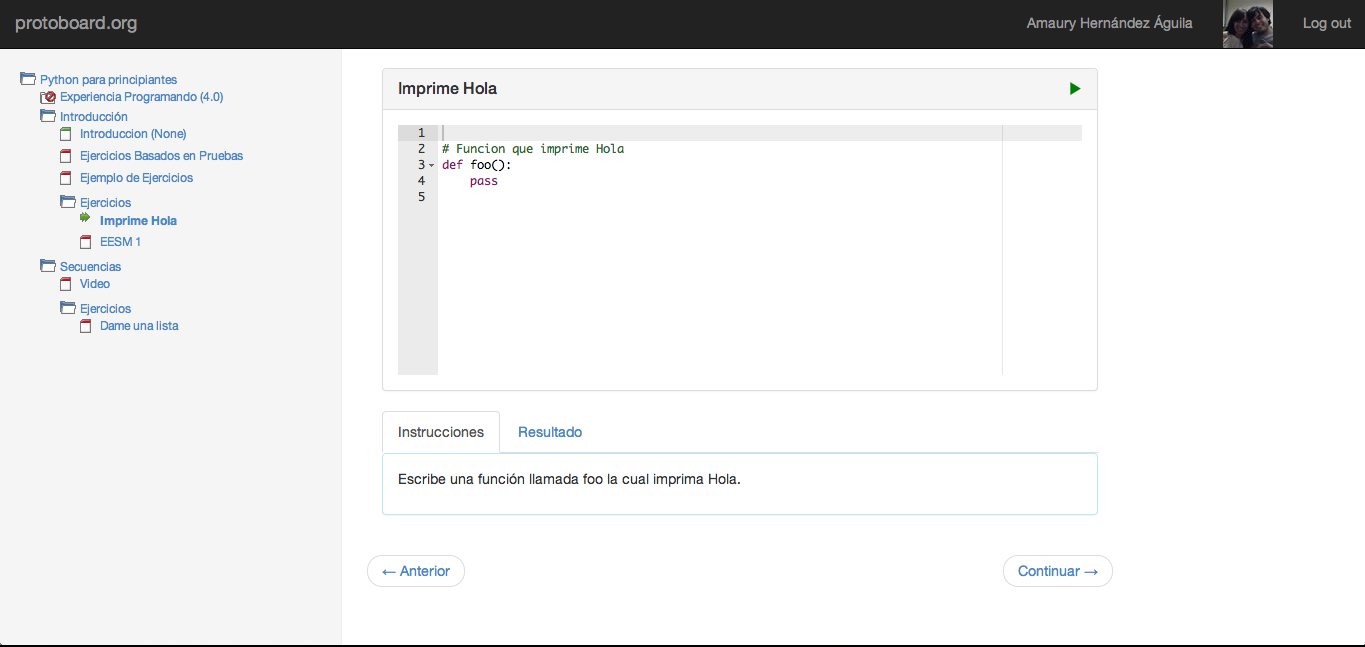
\includegraphics[width=16.09cm]{protoboard.png}} \caption{Interfaz gráfica
    de un curso en Protoboard
} \label{FigProtoboard}
\end{figure}

En la encuesta del método de muestreo de experiencia se presenta una
serie de seis preguntas, una por cada estado emocional que son de
interés para este trabajo: aburrimiento, relajación, entusiasmo,
concentración, distracción, y frustración. El estudiante, después de
haber resuelto un ejercicio, debe contestar esta encuesta de acuerdo a
cómo se sintió durante el ejercicio. Las preguntas se presentan con el
formato mostrado en la Figura \ref{FigESM}. En general, el estudiante
responde a la declaración "Me sentía frustrado/relajado/etc.'' usando
una escala Likert: muy de acuerdo, de acuerdo, neutral, en desacuerdo,
muy en desacuerdo. De esta forma, un usuario que no se haya sentido
para nada relajado durante su solución a un ejercicio, puede responden
"muy en desacuerdo'' a la declaración "Me sentía relajado''.

\begin{figure}[htp]
  \centerline{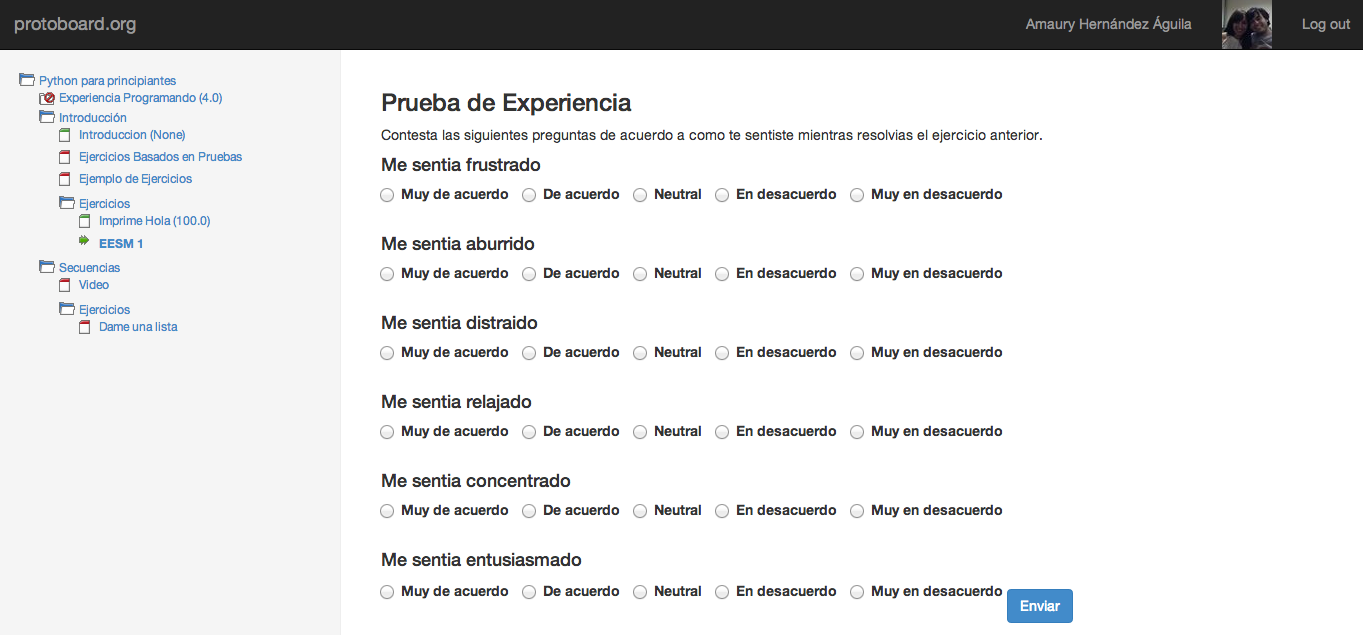
\includegraphics[width=16.09cm]{esm.png}} \caption{Encuesta de Método de
    Muestreo de Experiencia
} \label{FigESM}
\end{figure}

Para registrar la dinámica de tecleo y dinámica de ratón durante la
resolución de un ejercicio, se utilizaron las funciones mostradas en
el Algoritmo \ref{dinamica}. En general, cada vez que el usuario realiza
una pulsación de alguna tecla en el teclado o en el ratón, se registra
qué tecla fue pulsada, y en qué momento sucedió exactamente. El tiempo
es registrado en milisegundos transcurridos usando la función
Date().getTime() de Javascript. Adicionalmente, se registra todo
movimiento del ratón en intervalos de 100 milisegundos. Si el usuario
no ha realizado ningún movimiento en los próximos 100 milisegundos (en
otras palabras, si la posición en X y la posición en Y del ratón es la
misma que la de hace 100 milisegundos), no se registra ningún
movimiento. El código fuente completo se encuentra en el repositorio de
Protoboard en Github (https://github.com/mariosky/protoboard/).

\lstset{language=Java, breaklines=true, basicstyle=\footnotesize,  backgroundcolor=\color{mygray}}
\lstset{numbers=left, numberstyle=\tiny\color{red},
  keywordstyle=\color{blue}, rulecolor=\color{myblue},
  stringstyle=\color{mygreen}, title=\lstname ,  stepnumber=1, numbersep=-6pt}

\begin{lstlisting}[label=dinamica,frame=single]
$(document).keyup(function(evt) {
    keypresses.push(
	{"timestamp": new Date().getTime(),
         "keycode": evt.which,
	 "type": "keyup"});
});

$(document).keydown(function(evt) {
    keypresses.push(
	{"timestamp": new Date().getTime(),
         "keycode":evt.which,
	 "type": "keydown"});
});

$(document).mouseup(function(evt) {
    mousepresses.push(
	{"timestamp": new Date().getTime(),
         "mousecode": evt.which,
	 "type": "mouseup"});
});

$(document).mousedown(function(evt) {
    mousepresses.push(
	{"timestamp": new Date().getTime(),
         "mousecode":evt.which,
	 "type": "mousedown"});
});
\end{lstlisting}
\captionof{lstlisting}{Funciones para registrar la dinámica de ratón y
la dinámica de tecleo}

Para el preprocesamiento de los datos generados por el script de
Javascript presentado anteriormente, se creó un programa en Common
Lisp. El primer paso, después de extraer los datos del servidor web y
convertirlos a un formato legible por Common Lisp, es extraer todos
los dígrafos y trígrafos contenidos en las pulsaciones generadas por
los usuarios. Esta tarea resultó ser bastante complicada, y una parte
del proceso es mostrada en el Algoritmo \ref{extract-digraph} y el Algoritmo
\ref{extract-trigraph}. En general, el proceso consiste en determinar
cuáles son los 100 dígrafos y trígrafos más frecuentes dentro del
dataset total, y después se utilizan cada una de las funciones
encontradas en el Algoritmo \ref{feature-extraction}, para extraer las
características. Usando los 100 dígrafos y trígrafos más frecuentes,
se buscan cuáles de ellos estuvieron presentes en la resolución de un
ejercicio por parte de un usuario. Después se obtienen diferentes
métricas de éstos eventos presentes, por ejemplo, la duración entre el
evento key-down (presionar una tecla) de la primera tecla dentro de un
trígrafo, y el evento key-up (liberar una tecla) de la última tecla
dentro de ese mismo trígrafo. Para la mayoría de estas funciones para la
extracción de características se obtiene el promedio de los tiempos o
pulsaciones, y también se calcula la desviación estándar. El código
fuente completo se encuentra en el repositorio de Github
https://github.com/amherag/keyboard-mouse-dynamics.

Un dígrafo, en este contexto, significa cualquier combinación de dos
teclas realizadas por parte del usuario con el teclado de
computadora. Un trígrafo es similar, pero siendo una combinación de
tres teclas.

El curso de Python en Protoboard se dejó abierto durante varias
semanas y un total de 51 usuarios participaron, generando 142
registros. Esto significa que cada usuario en promedio realizó
cerca de 3 ejercicios de todo el curso de programación.

\lstset{language=Lisp, breaklines=true, basicstyle=\footnotesize,  backgroundcolor=\color{mygray}}
\lstset{numbers=left, numberstyle=\tiny\color{red},
  keywordstyle=\color{blue}, rulecolor=\color{myblue},
  stringstyle=\color{mygreen}, title=\lstname ,  stepnumber=1, numbersep=-6pt}

\begin{lstlisting}[frame=single]
\label{extract-digraph}
 (defun extract-digraphs (ks dgs)
  "Gets a list of all the 'popular' digraphs in a list of keypresses."
  (let ((result))
    (mapcar (lambda (dg)
              (maplist (lambda (k)
                         (push (digraph-subseq dg k) result)) ks)) dgs)
    (remove nil (nreverse result))
    ))

 (defun digraph-subseq (dg seq)
  "Used by extract-digraph"
  (when (and
         (string= (second (first seq)) "keydown")
         (= (caadr dg) (third (first seq)))
         (eql (cadadr dg)
            (third (find "keydown" (cdr seq) :test 'string= :key (lambda (elt)
                                                                   (second elt))))))
    (let ((sub nil))
      (block ntz
        (map nil (lambda (elt)
                   (push elt sub)
                     (when (has-digraph? (reverse sub) dg)
                       (return-from ntz (nreverse sub)))) seq)))))

 (defun has-digraph? (sub dg)
  "Used by (digraph-subseq)"
  (flet ((cdr-ks (elt) (cdr elt)))
    (let* ((kc1 (caadr dg))
           (kc2 (cadadr dg))
           (fst-dwn (remove `("keydown" ,kc1) sub :key #'cdr-ks :test 'equalp :count 1))
           (snd-dwn (remove `("keydown" ,kc2) fst-dwn :key #'cdr-ks :test 'equalp :count 1))
           (fst-up (remove `("keyup" ,kc1) snd-dwn :key #'cdr-ks :test 'equalp :count 1))
           (snd-up (remove `("keyup" ,kc2) fst-up :key #'cdr-ks :test 'equalp :count 1))
           (fst-kc? (and (= (third (first sub)) kc1) (string= "keydown" (second (first sub)))))
           (pos-kc1d (position `("keydown" ,kc1) sub :key #'cdr-ks :test 'equalp))
           (pos-kc1u (position `("keyup" ,kc1) sub :key #'cdr-ks :test 'equalp))
           (pos-kc2d (position `("keydown" ,kc2) sub :key #'cdr-ks :test 'equalp))
           (pos-kc2u (position `("keyup" ,kc2) sub :key #'cdr-ks :test 'equalp))
           (num-kd (count "keydown" sub :test 'string= :key (lambda (elt) (second elt))))
           )
      (if (and fst-kc?
               (= num-kd 2)
               (when (and (numberp pos-kc1d)
                          (numberp pos-kc1u)
                          (numberp pos-kc2d)
                          (numberp pos-kc2u))
                 (and (< pos-kc1d pos-kc2d)
                      (< pos-kc1d pos-kc1u)
                      (< pos-kc2d pos-kc2u)))
               (/= (length fst-dwn)
                   (length snd-dwn)
                   (length fst-up)
                   (length snd-up)))
          T))))
\end{lstlisting}
\captionof{lstlisting}{Función para determinar si una subsecuencia contiene a un dígrafo}


\begin{lstlisting}[frame=single]
\label{extract-trigraph}
 (defun extract-trigraphs (ks tgs)
  "Gets a list of all the 'popular' trigraphs in a list of keypresses."
  (let ((result))
    (mapcar (lambda (tg)
              (maplist (lambda (k)
                         (push (trigraph-subseq tg k) result)) ks)) tgs)
    (remove nil (nreverse result))
    ))

 (defun trigraph-subseq (tg seq)
  "Used by (extract-trigraphs)"
  (let* ((kc1 (first (cadr tg)))
         (kc2 (second (cadr tg)))
         (kc3 (third (cadr tg)))
         (snd-kd (let ((c 0))
                   (find '("keydown" 2) seq :test 'equalp :key 
                         (lambda (elt)
                           (when (string= "keydown" (second elt))
                             (incf c)
                             (list (second elt) c))
                           ))
                   ))
         (trd-kd (let ((c 0))
                   (find '("keydown" 3) seq :test 'equalp :key 
                         (lambda (elt)
                           (when (string= "keydown" (second elt))
                             (incf c)
                             (list (second elt) c))
                           ))
                   ))
         (fst-kc? (and (numberp kc1) (= (third (first seq)) kc1) (string= (second (first seq)) "keydown")))
         (snd-kc? (and snd-kd (numberp kc2) (= (third snd-kd) kc2)))
         (trd-kc? (and trd-kd (numberp kc3) (= (third trd-kd) kc3))))
    (when (and fst-kc? snd-kc? trd-kc?)
      (let ((sub nil))
        (block ntz
          (map nil (lambda (elt)
                     (push elt sub)
                     (when (has-trigraph? (reverse sub) tg)
                       (return-from ntz (nreverse sub)))) seq))))))

 (defun has-trigraph? (sub tg)
  "Used by (trigraph-subseq)"
  (flet ((cdr-ks (elt) (cdr elt)))
    (let* ((kc1 (first (cadr tg)))
           (kc2 (second (cadr tg)))
           (kc3 (third (cadr tg)))
           (fst-dwn (remove `("keydown" ,kc1) sub :key #'cdr-ks :test 'equalp :count 1))
           (snd-dwn (remove `("keydown" ,kc2) fst-dwn :key #'cdr-ks :test 'equalp :count 1))
           (trd-dwn (remove `("keydown" ,kc3) snd-dwn :key #'cdr-ks :test 'equalp :count 1))
           (fst-up (remove `("keyup" ,kc1) trd-dwn :key #'cdr-ks :test 'equalp :count 1))
           (snd-up (remove `("keyup" ,kc2) fst-up :key #'cdr-ks :test 'equalp :count 1))
           (trd-up (remove `("keyup" ,kc3) snd-up :key #'cdr-ks :test 'equalp :count 1))
           (fst-kc? (and (= (third (first sub)) kc1) (string= "keydown" (second (first sub)))))
           (pos-kc1d (position `("keydown" ,kc1) sub :key #'cdr-ks :test 'equalp))
           (pos-kc1u (position `("keyup" ,kc1) sub :key #'cdr-ks :test 'equalp))
           (pos-kc2d (position `("keydown" ,kc2) sub :key #'cdr-ks :test 'equalp))
           (pos-kc2u (position `("keyup" ,kc2) sub :key #'cdr-ks :test 'equalp))
           (pos-kc3d (position `("keydown" ,kc3) sub :key #'cdr-ks :test 'equalp))
           (pos-kc3u (position `("keyup" ,kc3) sub :key #'cdr-ks :test 'equalp))
           (num-kd (count "keydown" sub :test 'string= :key (lambda (elt) (second elt))))
           )
      (if (and fst-kc?
               (= num-kd 3)
               (when (and (numberp pos-kc1d)
                          (numberp pos-kc1u)
                          (numberp pos-kc2d)
                          (numberp pos-kc2u)
                          (numberp pos-kc3d)
                          (numberp pos-kc3u))
                 (and (< pos-kc1d pos-kc2d)
                      (< pos-kc2d pos-kc3d)
                      (< pos-kc1d pos-kc1u)
                      (< pos-kc2d pos-kc2u)
                      (< pos-kc3d pos-kc3u)))
               (/= (length fst-dwn)
                   (length snd-dwn)
                   (length fst-up)
                   (length snd-up)
                   (length trd-dwn)
                   (length trd-up)))
          T))))
\end{lstlisting}
\captionof{lstlisting}{Función para determinar si una subsecuencia
  contiene a un trígrafo}


\begin{lstlisting}[frame=single]
\label{feature-extraction}
;;
;; Feature extracting functions
;;

 (defun 2G-1D2D (dgs)
  (let ((times-lst (mapcar (lambda (dg)
            (let ((fst-kd (first dg))
                  (snd-kd (find "keydown" dg :test 'string= :key (lambda (elt) (second elt)) :from-end t)))
              (- (first snd-kd) (first fst-kd)))) dgs)))
    `((:mean ,(mean times-lst)) (:sd ,(sd times-lst)))))

;;(time (2G-1D2D (extract-digraphs *la *dgs)))

 (defun 2G-1Dur (dgs)
  (let ((times-lst (mapcar (lambda (dg)
            (let* ((fst-kd (first dg))
                   (fst-ku (find `("keyup" ,(third fst-kd)) dg :test 'equalp :key (lambda (elt) (cdr elt)))))
              (- (first fst-ku) (first fst-kd)))) dgs)))
    `((:mean ,(mean times-lst)) (:sd ,(sd times-lst)))))

;;(time (2G-1Dur (extract-digraphs *la *dgs)))

 (defun 2G-1KeyLat (dgs)
  (let ((times-lst (mapcar (lambda (dg)
                             (let* ((fst-kd (first dg))
                                    (fst-ku (find `("keyup" ,(third fst-kd)) dg :test 'equalp :key (lambda (elt) (cdr elt))))
                                    (pos-fst-ku (position `("keyup" ,(third fst-kd)) dg :test 'equalp :key (lambda (elt) (cdr elt))))
                                   (nxt-kd (find "keydown" (subseq dg (1+ pos-fst-ku)) :test 'string= :key (lambda (elt) (second elt)))))
                               (if (null (first nxt-kd))
                                   0
                                   (- (first nxt-kd) (first fst-ku)))
                               )) dgs)))
    `((:mean ,(mean times-lst)) (:sd ,(sd times-lst)))))

;;(time (2G-1KeyLat (extract-digraphs *la *dgs)))

 (defun 2G-2Dur (dgs)
       (let ((times-lst (mapcar (lambda (dg)
                                  (let* (
                                        (snd-kd (find "keydown" dg :test 'string= :key (lambda (elt) (second elt)) :from-end t))
                                        (snd-ku (find `("keyup" ,(third snd-kd)) dg
                                                      :test 'equalp :key (lambda (elt) (cdr elt)) :from-end t)))
                                    (- (first snd-ku) (first snd-kd)))) dgs)))
         `((:mean ,(mean times-lst)) (:sd ,(sd times-lst)))))

;;(time (2G-2Dur (extract-digraphs *la *dgs)))

 (defun 2G-Dur (dgs)
  (let ((times-lst (mapcar (lambda (dg)
            (let ((fst-kd (first dg))
                  (snd-ku (find "keyup" dg :test 'string= :key (lambda (elt) (second elt)) :from-end t)))
              (- (first snd-ku) (first fst-kd)))) dgs)))
    `((:mean ,(mean times-lst)) (:sd ,(sd times-lst)))))

;;(time (2G-Dur (extract-digraphs *la *dgs)))

 (defun 2G-NumEvents (dgs)
  (let ((numevents-lst (mapcar (lambda (dg)
                             (length dg)) dgs)))
    `((:mean ,(mean numevents-lst)) (:sd ,(sd numevents-lst)))))

;;(time (2G-NumEvents (extract-digraphs *la *dgs)))

 (defun 3G-1D2D (tgs)
  (let ((times-lst (mapcar (lambda (tg)
            (let ((fst-kd (first tg))
                  (snd-kd (find "keydown" (cdr tg) :test 'string= :key (lambda (elt) (second elt)))))
              (- (first snd-kd) (first fst-kd)))) tgs)))
    `((:mean ,(mean times-lst)) (:sd ,(sd times-lst)))))

;;(time (3G-1D2D (extract-trigraphs *la *tgs)))

 (defun 3G-1Dur (tgs)
  (let ((times-lst (mapcar (lambda (tg)
            (let* ((fst-kd (first tg))
                   (fst-ku (find `("keyup" ,(third fst-kd)) tg :test 'equalp :key (lambda (elt) (cdr elt)))))
              (- (first fst-ku) (first fst-kd)))) tgs)))
    `((:mean ,(mean times-lst)) (:sd ,(sd times-lst)))))

;;(time (3G-1Dur (extract-trigraphs *la *tgs)))

 (defun 3G-1KeyLat (tgs)
  (let ((times-lst (mapcar (lambda (tg)
                             (let* (
                                    (fst-kd (first tg))
                                    (fst-ku (find `("keyup" ,(third fst-kd)) tg :test 'equalp :key (lambda (elt) (cdr elt))))
                                    (pos-fst-ku (position `("keyup" ,(third fst-kd)) tg :test 'equalp :key (lambda (elt) (cdr elt))))
                                    (nxt-kd (find "keydown" (subseq tg (1+ pos-fst-ku)) :test 'string= :key (lambda (elt) (second elt)))))
                               (if (null (first nxt-kd))
                                   0
                                   (- (first nxt-kd) (first fst-ku)))
                               )) tgs)))
    `((:mean ,(mean times-lst)) (:sd ,(sd times-lst)))))

;;(time (3G-1KeyLat (extract-trigraphs *la *tgs)))

 (defun 3G-2D2D (tgs)
  (let ((times-lst (mapcar (lambda (tg)
            (let ((snd-kd (find "keydown" (cdr tg) :test 'string= :key (lambda (elt) (second elt))))
                  (trd-kd (find "keydown" tg :test 'string= :key (lambda (elt) (second elt)) :from-end t)))
              (- (first trd-kd) (first snd-kd)))) tgs)))
    `((:mean ,(mean times-lst)) (:sd ,(sd times-lst)))))

;;(time (3G-2D2D (extract-trigraphs *la *tgs)))

 (defun 3G-2Dur (tgs)
  (let ((times-lst (mapcar (lambda (tg)
            (let* ((snd-kd (find "keydown" (cdr tg) :test 'string= :key (lambda (elt) (second elt))))
                   (snd-ku (find `("keyup" ,(third snd-kd)) tg :test 'equalp :key (lambda (elt) (cdr elt)))))
              (- (first snd-ku) (first snd-kd)))) tgs)))
    `((:mean ,(mean times-lst)) (:sd ,(sd times-lst)))))

;;(time (3G-2Dur (extract-trigraphs *la *tgs)))

 (defun 3G-2KeyLat (tgs)
  (let ((times-lst (mapcar (lambda (tg)
                             (let* ((snd-ku (let ((c 0))
                                              (find '("keyup" 2) tg :test 'equalp :key 
                                                    (lambda (elt)
                                                      (when (string= "keyup" (second elt))
                                                        (incf c)
                                                        (list (second elt) c))))))
                                    (pos-snd-ku (let ((c 0))
                                              (position '("keyup" 2) tg :test 'equalp :key 
                                                    (lambda (elt)
                                                      (when (string= "keyup" (second elt))
                                                        (incf c)
                                                        (list (second elt) c))))))

                                    (nxt-kd (let ((c 0))
                                                  (find '("keydown" 3) tg :test 'equalp :key 
                                                            (lambda (elt)
                                                              (when (string= "keydown" (second elt))
                                                                (incf c)
                                                                (list (second elt) c))))))
                                    (pos-nxt-kd (let ((c 0))
                                                  (position '("keydown" 3) tg :test 'equalp :key 
                                                            (lambda (elt)
                                                              (when (string= "keydown" (second elt))
                                                                (incf c)
                                                                (list (second elt) c)))))))
                               (if (or (null (first nxt-kd)) (< pos-nxt-kd pos-snd-ku))
                                   0
                                   (- (first nxt-kd) (first snd-ku))))) tgs)))
    `((:mean ,(mean times-lst)) (:sd ,(sd times-lst)))))

;;(time (3G-2KeyLat (extract-trigraphs *la *tgs)))

 (defun 3G-3Dur (tgs)
  (let ((times-lst (mapcar (lambda (tg)
                             (let* ((trd-kd (let ((c 0))
                                              (find '("keydown" 3) tg :test 'equalp :key 
                                                    (lambda (elt)
                                                      (when (string= "keydown" (second elt))
                                                        (incf c)
                                                        (list (second elt) c))))))
                                    (pos-trd-kd (let ((c 0))
                                              (position '("keydown" 3) tg :test 'equalp :key 
                                                    (lambda (elt)
                                                      (when (string= "keydown" (second elt))
                                                        (incf c)
                                                        (list (second elt) c))))))
                                    (trd-ku (find `("keyup" ,(third trd-kd)) (subseq tg (1+ pos-trd-kd))
                                                  :test 'equalp :key (lambda (elt) (cdr elt)))))
                                   (- (first trd-ku) (first trd-kd)))) tgs)))
    `((:mean ,(mean times-lst)) (:sd ,(sd times-lst)))))

;;(time (3G-3Dur (extract-trigraphs *la *tgs)))

 (defun 3G-Dur (tgs)
  (let ((times-lst (mapcar (lambda (tg)
            (let* ((fst-kd (first tg))
                   (trd-ku (car (last tg))))
              (- (first trd-ku) (first fst-kd)))) tgs)))
    `((:mean ,(mean times-lst)) (:sd ,(sd times-lst)))))

;;(time (3G-Dur (extract-trigraphs *la *tgs)))

 (defun 3G-NumEvents (tgs)
  (let ((numevents-lst (mapcar (lambda (tg)
                             (length tg)) tgs)))
    `((:mean ,(mean numevents-lst)) (:sd ,(sd numevents-lst)))))

;;(time (3G-NumEvents (extract-trigraphs *la *tgs)))

;;
;; Non-Graph Keystroke Features
;;

 (defun NumBackspaces (ks)
  (let ((c 0))
    (map nil (lambda (k)
               (when (= (third k) 8)
                 (incf c))) ks)
    c))

;;(NumBackspaces *ks)

 (defun NumKeystrokes (ks)
  (count "keydown" ks :test 'string= :key (lambda (elt) (second elt))))

;;(NumKeystrokes *ks)

 (defun ActivityTime (ks)
  (- (caar (last ks))
     (caar ks)))

;;(ActivityTime *ks)

;;
;; Mouse Dynamics Features
;;

 (defun MousePressesDur (mps)
  "Deltas between each mousepress. Mean and Standard Deviation as result."
  (let ((deltas (remove nil (maplist (lambda (mp)
                                       (when (and (second mp)
                                                  (string= "mousedown" (second (first mp)))
                                                  (string= "mouseup" (second (second mp))))
                                         (- (car (second mp))
                                            (car (first mp))))) mps))))
    `((:mean ,(mean deltas)) (:sd ,(sd deltas)))))

;;(MousePressesDur *mps)

 (defun MouseMovementDur (mms)
  (let ((deltas (remove nil (maplist (lambda (mm)
                                       (when (second mm)
                                         (let ((delta (- (car (second mm))
                                                         (car (first mm)))))
                                           (when (> delta 150)
                                             delta)))) mms))))
    `((:mean ,(mean deltas)) (:sd ,(sd deltas)))))

;;(MouseMovementDur *mms)

 (defun MouseMovementX (mms)
  (let ((deltas (remove nil (maplist (lambda (mm)
                                       (when (second mm)
                                         (abs (- (cadr (second mm))
                                                 (cadr (first mm)))))) mms))))
    `((:mean ,(mean deltas)) (:sd ,(sd deltas)))))

;;(MouseMovementX *mms)

 (defun MouseMovementY (mms)
  (let ((deltas (remove nil (maplist (lambda (mm)
                                       (when (second mm)
                                         (abs (- (caddr (second mm))
                                                 (caddr (first mm)))))) mms))))
    `((:mean ,(mean deltas)) (:sd ,(sd deltas)))))

\end{lstlisting}
\captionof{lstlisting}{Funciones para extraer las características
  basadas en dígrafos y trígrafos, así como dinámica de ratón}





\begin{lstlisting}[frame=single]

 (defun csv (final)
  (with-open-file (str "~/thesis.csv" :direction :output :if-exists :supersede :if-does-not-exist :create)
    (format str (apply #'concatenate 'string "2G_1D2D_MEAN,2G_1D2D_SD,2G_1Dur_MEAN,2G_1Dur_SD,2G_1KeyLat_MEAN,2G_1KeyLat_SD,2G_2Dur_MEAN,2G_2Dur_SD,2G_Dur_MEAN,2G_Dur_SD,2G_NumEvents_MEAN,2G_NumEvents_SD,3G_1D2D_MEAN,3G_1D2D_SD,3G_1Dur_MEAN,3G_1Dur_SD,3G_1KeyLat_MEAN,3G_1KeyLat_SD,3G_2D2D_MEAN,3G_2D2D_SD,3G_2Dur_MEAN,3G_2Dur_SD,3G_2KeyLat_MEAN,3G_2KeyLat_SD,3G_3Dur_MEAN,3G_3Dur_SD,3G_Dur_MEAN,3G_Dur_SD,3G_NumEvents_MEAN,3G_NumEvents_SD,Mouse_Presses_Dur_MEAN,Mouse_Presses_Dur_SD,Mouse_Movement_Dur_MEAN,Mouse_Movement_Dur_SD,Mouse_Movement_X_MEAN,Mouse_Movement_X_SD,Mouse_Movement_Y_MEAN,Mouse_Movement_Y_SD,Attempts,Frustration,Boredom,Distraction,Relaxation,Focus,Excitement
"
         (remove nil (mapcar (lambda (f)
                               (if (and (= (length f) 40) (not (some #'null f)) (not (null (car (last f)))))
                                   (format nil "~{~a,~}~{~a~^,~}~%" (subseq f 0 39) (car (last f))))) final))))))

 (defun final (exercises)
  (mapcar (lambda (e)
            (let* ((ula (prune-la (decode-json-from-string (clean-pythons-json (caar (first e))))))
                   (eesm (prune-eesm (decode-json-from-string (clean-pythons-json (caaadr e)))))
                   (ks (preproc-keystrokes ula))
                   (mms (preproc-mousemovement ula))
                   (mps (preproc-mousepresses ula))
                   (attempts (third e)))
              ;;(error ula)
              ;;(error ks)
              (append
               (when ks
                 (let ((dgs (extract-digraphs ks *dgs))
                       (tgs (extract-trigraphs ks *tgs)))
                   (if (and dgs tgs)
                     (list
                      ;;(error ks)
                  (cadr (assoc :mean (2G-1D2D dgs)))
                  (cadr (assoc :sd (2G-1D2D dgs)))
                  (cadr (assoc :mean (2G-1Dur dgs)))
                  (cadr (assoc :sd (2G-1Dur dgs)))
                  (cadr (assoc :mean (2G-1KeyLat dgs)))
                  (cadr (assoc :sd (2G-1KeyLat dgs)))
                  (cadr (assoc :mean (2G-2Dur dgs)))
                  (cadr (assoc :sd (2G-2Dur dgs)))
                  (cadr (assoc :mean (2G-Dur dgs)))
                  (cadr (assoc :sd (2G-Dur dgs)))
                  (cadr (assoc :mean (2G-NumEvents dgs)))
                  (cadr (assoc :sd (2G-NumEvents dgs)))

                  (cadr (assoc :mean (3G-1D2D tgs)))
                  (cadr (assoc :sd (3G-1D2D tgs)))
                  (cadr (assoc :mean (3G-1Dur tgs)))
                  (cadr (assoc :sd (3G-1Dur tgs)))
                  (cadr (assoc :mean (3G-1KeyLat tgs)))
                  (cadr (assoc :sd (3G-1KeyLat tgs)))
                  (cadr (assoc :mean (3G-2D2D tgs)))
                  (cadr (assoc :sd (3G-2D2D tgs)))
                  (cadr (assoc :mean (3G-2Dur tgs)))
                  (cadr (assoc :sd (3G-2Dur tgs)))
                  (cadr (assoc :mean (3G-2KeyLat tgs)))
                  (cadr (assoc :sd (3G-2KeyLat tgs)))
                  (cadr (assoc :mean (3G-3Dur tgs)))
                  (cadr (assoc :sd (3G-3Dur tgs)))
                  (cadr (assoc :mean (3G-Dur tgs)))
                  (cadr (assoc :sd (3G-Dur tgs)))
                  (cadr (assoc :mean (3G-NumEvents tgs)))
                  (cadr (assoc :sd (3G-NumEvents tgs)))
                  )
                     '(NIL))))
               (when mps
                 (list
                  (cadr (assoc :mean (MousePressesDur mps)))
                  (cadr (assoc :sd (MousePressesDur mps)))
                  ))
               (when mms
                 ;;(error mms)
                (list
                 (cadr (assoc :mean (MouseMovementDur mms)))
                 (cadr (assoc :sd (MouseMovementDur mms)))
                 (cadr (assoc :mean (MouseMovementX mms)))
                 (cadr (assoc :sd (MouseMovementX mms)))
                 (cadr (assoc :mean (MouseMovementY mms)))
                 (cadr (assoc :sd (MouseMovementY mms)))
              ))
               (list attempts)
               (list eesm)
              )
              )) exercises))
\end{lstlisting}
\captionof{lstlisting}{Función para determinar si una subsecuencia
  contiene a un trígrafo}